\documentclass{../../../fal_assignment}
\graphicspath{ {../../../} }

\usepackage{url}
\usepackage{graphicx}
\usepackage{amsmath}
\usepackage{varwidth}
\usepackage{xcolor}
\usepackage{algorithm}
\usepackage{algpseudocode}
\usepackage{listings}
\lstset{
	basicstyle=\footnotesize\ttfamily,
	tabsize=4,
	showstringspaces=false,
	breaklines=true,
	prebreak={\space\hbox{\textcolor{Gray}{$\hookleftarrow$}}},
	language=C++
}
\usepackage{enumitem}

\usepackage{tikz}
\usetikzlibrary{shapes.geometric, arrows}

\tikzstyle{flowchartnode} = [rectangle, minimum height=0.8cm, text centered, text width=3cm, draw=black, font=\small]
\tikzstyle{startstop} = [flowchartnode, rounded corners=0.4cm]
\tikzstyle{process} = [flowchartnode]
\tikzstyle{io} = [flowchartnode, trapezium, trapezium left angle=70, trapezium right angle=110, text width=2cm]
\tikzstyle{decision} = [flowchartnode, diamond, aspect=2, text width=2cm]
\tikzstyle{arrow} = [thick,->,>=stealth]

\title{COMP140 Worksheet B: Mandelbrot set}
\author{Brian McDonald \& Ed Powley}


\begin{document}

\maketitle

In this worksheet, you will use the SDL2 library (\url{https://www.libsdl.org/index.php}) to write a program to generate and display the \emph{Mandelbrot set} fractal; see Figure~\ref{fig:mandelbrot}.
This fractal colours each pixel of the image according to an iterated mathematical formula, as described below.
The GitHub repository contains a project named \texttt{Mandelbrot} for you to build upon.
This contains code to create and display a blank image; you will implement the calculations to generate the Mandelbrot set fractal.

\begin{figure}[!h]
	\begin{center}
		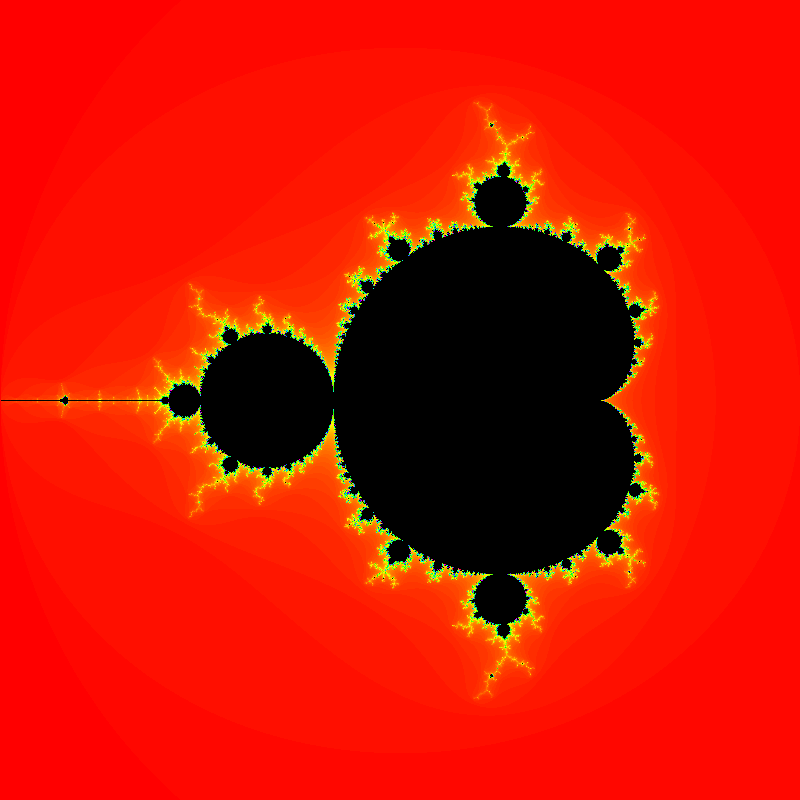
\includegraphics[width=0.6\textwidth]{mandelbrot.png}
	\end{center}
	\caption{The Mandelbrot set fractal.}
	\label{fig:mandelbrot}
\end{figure}

\section{} \label{core-c-first}

To generate an interesting fractal, the on-screen $x$ and $y$ coordinates must first be rescaled.
In the skeleton project the pixel coordinates range from $0$ to $800$,
whereas the Mandelbrot set fractal is most interesting in the region $-2 \leq x \leq 1$ and $-1.5 \leq y \leq 1.5$.

Let $p_x$ be the $x$ coordinate of the pixel. This can be remapped into the range $x_{\text{min}}$ to $x_{\text{max}}$ using the following formula:
\begin{equation*}
x_0 = \frac{p_x}{\text{image.width}} \times \left( x_{\text{max}} - x_{\text{min}} \right) + x_{\text{min}}
\end{equation*}
The $y$ coordinate can be remapped using a similar formula.

\textbf{Implement} the above calculations for the $x$ and $y$ coordinates, at the indicated parts of \texttt{Mandelbrot.cpp}.

\section{} \label{core-c-last}

The Mandelbrot set is based on the following sequence of numbers. Let $x_0$ and $y_0$ be the coordinates of a point in the image.
Then the sequence $x_1, y_1, x_2, y_2, x_3, y_3, \dots$ is defined\footnote{%
	If you are familiar with complex numbers, you may notice that this is equivalent to $z_{j+1} = z_j^2 + z_0$, where $z_j = x_j + y_j i$.
} recursively for $i = 0, 1, 2, 3, \dots$ by:

\begin{align*}
x_{i+1} &= (x_i)^2 - (y_i)^2 + x_0 \\
y_{i+1} &= (2 \times x_i \times y_i) + y_0 \\
\end{align*}

The points are coloured according to the \emph{smallest} value of $i$ for which $(x_i)^2 + (y_i)^2 \geq 4$.
If such a value of $i$ is not found after a large number of iterations (for example $i=200$), the pixel is coloured black.

\textbf{Implement} an algorithm which performs the above computation, determining the smallest value of $i$
for which $(x_i)^2 + (y_i)^2 \geq 4$ and selecting the appropriate pixel colour.
Implement the algorithm in \texttt{Mandelbrot.cpp} so that the program generates the Mandelbrot set fractal (Figure~\ref{fig:mandelbrot}) when it is run.

\section{Stretch goal} \label{stretch-c}

Mathematicians have discovered many other fractals besides the Mandelbrot set.

\textbf{Research} a different type of fractal, using online resources and/or academic literature.
Briefly summarise your findings (with URLs and/or citations) in your \texttt{readme.md} file.

\textbf{Implement} a generator for the fractal you have researched.
Allow the user to choose (by command line entry) which fractal they want to generate when the program starts up: the Mandelbrot set or the new fractal.
You may wish to restructure the skeleton program to accommodate the new fractal generation algorithm.
\section*{Submission instructions}

Begin by \textbf{forking} the GitHub repository at the following URL:

\url{https://github.com/Falmouth-Games-Academy/comp140-worksheetB}

You should complete a pull request before the hand-in on Friday by 5pm on Week 3. Feedback will be given in the pull request and in class.
	
\section*{Marking criteria}
	
	Remember that \textbf{it is better to submit incomplete work than to submit nothing at all}. 
	
	To demonstrate \textbf{basic competency}, complete the following:
	\begin{itemize}
		\item \textbf{Timely Submission:} Obtain the marks for timely submission, you must submit (as a GitHub pull request).
		As with other worksheets, you may resubmit after these deadlines in order to collect extra correctness or quality marks.
		This is awarded as long as you submit \emph{something} for each part by the deadline,
		even if your submission has bugs or other issues.
	\end{itemize} 
	
	To demonstrate \textbf{basic proficiency}, complete the following:
	\begin{itemize}
		\item \textbf{Achieve basic competency}
		\item \textbf{Complete} Algorithm \ref{core-c-first}. \textbf{Note:} You will not be penalised for trivial errors which do not
		affect the overall functioning of your programs
		\item Appropriate use of GitHub, with descriptive commit messages 
		\item Comments are used where appropriate, and are well written.
	\end{itemize}
	
	To demonstrate \textbf{novice competency}, complete the following:
	\begin{itemize}
		\item Achieve \textbf{basic proficiency}
		\item \textbf{Complete} Algorithm \ref{core-c-last}. \textbf{Note:} You will not be penalised for trivial errors which do not
		affect the overall functioning of your programs
		\item Your code is well formatted. Variable and function names are clear and descriptive.
	\end{itemize}
	
	To demonstrate \textbf{novice proficiency}, complete the following:
	\begin{itemize}
		\item Achieve \textbf{novice competency}
		\item \textbf{Research} a different fractal
	\end{itemize}
	
	To demonstrate \textbf{professional competency}, complete the following:
	\begin{itemize}
		\item Achieve \textbf{novice proficiency}
		\item \textbf{Implement} a new fractal and allow the user to choose what fractal to generate
	\end{itemize}
	
	
\end{document}
